\chapter{Reducibility of Representations, I}
\label{ch-reducibility1}

This chapter is based on Joshi's book Ref.\cite{Joshi-book}.

Representations (reps) of groups are defined in Section \ref{sec-def-rep}.
In this chapter, we will discuss
 reps of finite groups in more detail.




\begin{figure}[h!]
\centering
\includegraphics[width=6in]
{reducibility1/syms-square.png}
\caption{Symmetries of a square.
The operators $N_i$ for $i=1,2$
replace $i$'th component
by its negative. The operator $S_{12}$
swaps components 1 and 2. Ref.\cite{Joshi-book}
uses $m_x=N_2$, $m_y=N_1$, $\s_\mu=\s_{y=-x}$,
$\s_\nu=\s_{y=x}$.
$(x,y)$ maps to whatever it says under each square.}
\label{fig-syms-square}
\end{figure}

Fig.\ref{fig-syms-square}
shows an 8 order group $\sqgroup$\footnote{Joshi Ref.\cite{Joshi-book} calls this group $C_{4\nu}$} of symmetries of
a square. The group is generated by the 3 generators
$N_1$, $N_2$ and $S_{2}$. (i.e., every group element is of the form $N_1^a N_2^b S_{12}^c$,
for $a,b,c\in\ZZ_{>0}$.

\beq
[N_1, N_2]=0, \quad \begin{pmatrix}N_1\\N_2\end{pmatrix}
S_{12}=S_{12}\begin{pmatrix}N_2\\N_1\end{pmatrix}, \quad
N_1^2=N_2^2=S_{12}^2=1
\eeq

Using these simple-to-remember identities,
we could easily calculate a
\qt{multiplication table} for $\sqgroup$.
(i.e. a table with all the elements of the group
as column and row labels, and with 
the product $ab$ as entry 
for row $a$ and column $b$). We won't do so here but
you can find it in Ref.\cite{Joshi-book}.

Rearrangement theorem: $aG=a$ for a group $G$ and 
$a\in G$.

Conjugacy classes (CC) are defined in Chapter  \ref{ch-lagranges-theorem}.
The CCs of $\sqgroup$ are 
given in Fig.\ref{fig-cc-sqgroup}.
\begin{figure}
\begin{tabular}{l}
\\ $CC_1=(E)$
\\ $CC_2=(N_1 S_{12}, N_2 S_{12})$ (rotations  by $90$ and $270$ degrees)
\\ $CC_3=(N_1N_2)$ (rotation by 180 degrees)
\\ $ CC_4=(N_1, N_2)$ (refection about $x$ or $y$ axis)
 \\ $CC_5=(S_{12}, N_1N_2 S_{12})$ (reflection about $y=x$ or $y=-x$ diagonals)
\end{tabular}
\caption{CCs for $\sqgroup$}
\label{fig-cc-sqgroup}
\end{figure}

multiplication of classes

\beq
CC_i CC_j =\{ ab\mid a\in CC_i, b\in CC_j\}
\eeq

\beq
CC_i CC_j =\sum_k a^k_{ij}CC_k
\eeq
where $a^k_{ij}\in \ZZ_{>0}$.

Suppose $S$ (smaller) and $L$ (larger) are two vector spaces and $S\subset L$, with $L\neq S$ (i.e., proper subspace). Suppose $\calg$ is a group.
Suppose $\calg S\subset S$ and $\calg L  \subset L$. Then  we say $S$ is an
{\bf invariant subspace} of $L$ under $\calg$,
and we say  $L$ is {\bf reducible} under $\calg$.

\begin{claim}
Suppose $S$ is an invariant subspace of $L$ under $\calg$. Then for any rep $(L, \rho_L)$ of $\calg$, we must have

\beq
\rho_L(g)=
\begin{array}{r|cc}
&S&S^c
\\
\hline
S&A^{d_S\times d_S}&0
\\S^c&C^{d_{S^c}\times d_S}& D^{d_{S^c}\times d_{S^c}}
\end{array}
\label{eq-redu-mat}
\eeq
for all $g\in \calg$,
where $S^c=L-S$, $d_S=$ dimension of vector space $S$, $d_{S^c}=$ dimension of vector space $S^c$.
Furthermore, if $\rho_L()$ is a unitary rep,
then

\beq
C^{d_{S^c}\times d_S}=0
\eeq


\end{claim}
\proof

The zero matrix in \ref{eq-redu-mat}
follows because $\calg S\subset S$.
Note that 
if

\beq
\rho_L(g_1)=
\begin{pmatrix}
A_1&0
\\
C_1&D_1
\end{pmatrix},\quad
\rho_L(g_2)=
\begin{pmatrix}
A_2&0
\\
C_2&D_2
\end{pmatrix}
\eeq
then

\beq
\rho_L(g_1)\rho_L(g_2)=
\begin{pmatrix}
A_1 A_2&0
\\
X & D_1 D_2
\end{pmatrix}
\eeq
where

\beq X=C_1 A_2 + D_1 C_2 \eeq
If
$\rho()$ is a unitary rep,
then $X=0$ because the rows of 
the full matrix must yield $d_L$
orthonormal vectors and the columns must too.
This is possible only if $X=0$.

If $X=0$, we can define unitary reps $\rho_S$ and $\rho_{S^c}$ so that

\beq
\rho_S(g_1)=A_1,\quad \rho_S(g_2)=A_2,\quad
\rho_S(g_1 g_2)=A_1 A_2
\eeq

\beq
\rho_{S^c}(g_1)=D_1,\quad \rho_{S^c}(g_2)=D_2,\quad
\rho_{S^c}(g_1 g_2)=D_1 D_2
\eeq
\qed

\begin{claim}
For any representation $\rho()$,
there is an equivalent unitary rep $\hat{\rho}()$.
\end{claim}
\proof

Define the Hermitian matrix $H$ by

\beq
H=\sum_{g\in\calg}\rho(g)\rho^\dagger(g)
\eeq

Find a unitary matrix $U$ that diagonalizes $H$:

\beqa
H_d &=& U^\dagger H U
\\
&=&
U^\dagger\left[
\sum_{g\in\calg}\rho(g)\rho^\dagger(g)
\right]
U
\eeqa
where $H_d$ is a diagonal matrix.


Define a new rep $\rho_1()$ by

\beq
\rho_1(g)= U^\dagger \rho(g) U
\eeq
for all $g\in\calg$.

Note that  
\beq
H_d =\sum_{g\in\calg }\rho_1(g)\rho_1^\dagger(g)
\eeq

Note that the diagonal elements of $H_d$
must be positive.
Indeed,

\beqa
(H_d)_{kk} &=&
 \sum_{g\in\calg}\sum_j
[\rho_1(g)]_{kj}[\rho_1^*(g)]_{kj}
\\\
&=&
\sum_{g\in\calg}\sum_j 
\left|[\rho_1(g)]_{kj}\right|^2
\\
&\geq& 0
\eeqa
Actually, the diagonal elements of
$H_d$ must be strictly positive
because if the $k$th one were zero,
the $k$ row of $\rho_1(g)$ would be zero
for all $g\in\calg$. So all 
$\rho_1(g)$ would have a zero
determinant. 
Then all $\rho(g)$
would have a zero determinant and no inverse.
Then the rep $\rho()$
that we started would not
be valid, in contradiction
with the premise of the claim.

Now define

\beq
\hat{\rho}(g)=
H_d^{-\frac{1}{2}}
\rho_1(g)H_d^{\frac{1}{2}}
\eeq
for $g\in \calg$. 

Finally, check that $\hat{\rho}(g)$ is unitary
for all $g\in\calg$.

\beqa
\hat{\rho}(g)
\hat{\rho}^\dagger(g)
&=&
H_d^{-\frac{1}{2}}
\rho_1(g)
H_d
\rho_1^\dagger(g)
H_d^{-\frac{1}{2}}
\\
&=&
H_d^{-\frac{1}{2}}
\rho_1(g)
\left[
\sum_{g'\in\calg }\rho_1(g')\rho_1^\dagger(g')
\right]
\rho_1^\dagger(g)
H_d^{-\frac{1}{2}}
\\
&=&
H_d^{-\frac{1}{2}}
\left[
\sum_{g'\in\calg }\rho_1(gg')\rho_1^\dagger(gg')
\right]
H_d^{-\frac{1}{2}}
\\
&=&
H_d^{-\frac{1}{2}}
\left[
H_d
\right]
H_d^{-\frac{1}{2}}
\\
&=& 1
\eeqa
\qed